\begin{frame}{What is a Program Specification?}
    \begin{block}{The Contract}
        A program specification acts as a formal contract. It precisely describes the expected behavior of a piece of code.
        \begin{itemize}
            \item It does \textbf{not} describe \emph{how} the program works.
            \item It \textbf{does} describe \emph{what} the program must accomplish.
        \end{itemize}
    \end{block}
    \begin{block}{Key Components}
        A specification consists of two main parts:
        \begin{itemize}
            \item \textbf{Precondition:} A condition that must be true \emph{before} the program is executed.
            \item \textbf{Postcondition:} A condition that is guaranteed to be true \emph{after} the program terminates.
        \end{itemize}
    \end{block}
\end{frame}

\begin{frame}{Visualizing a Specification}
    \framesubtitle{From Initial to Final State}
    \begin{center}
        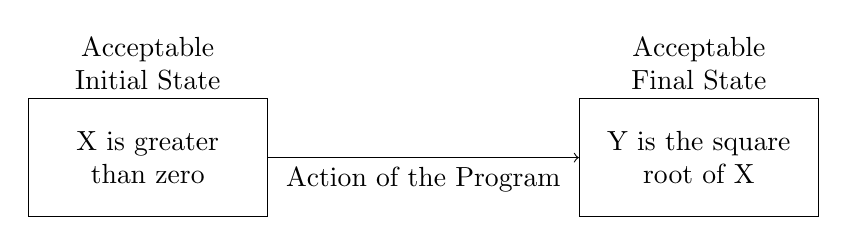
\begin{tikzpicture}
            % Define style for the boxes
            \tikzstyle{statebox} = [draw, rectangle, minimum height=1.5cm, text width=2.8cm, align=center]

            % Nodes for states
            \node [statebox] (initial) at (-1,0) {X is greater than zero};
            \node [statebox] (final) at (6,0) {Y is the square root of X};

            % Labels above the states
            \node [align=center] at (-1,1.2) {Acceptable \\ Initial State};
            \node [align=center] at (6,1.2) {Acceptable \\ Final State};

            % Arrow with label for the program's action
            \draw [->] (initial) -- node[below, align=center] {Action of the Program} (final);
        \end{tikzpicture}
    \end{center}
\end{frame}

\begin{frame}{The Precondition (P)}
    \begin{block}{Acceptable Initial State}
        The \textbf{precondition} defines the set of initial states for which the program is guaranteed to work correctly.
        \begin{itemize}
            \item It's an assumption about the values of program variables before execution.
            \item If the precondition is not met, the program has no obligations. It can crash, loop forever, or produce a wrong answer.
            \item Note: Reasoning about memory layout and heap requires \emph{Separation Logic}, an extension of Hoare Logic.
        \end{itemize}
    \end{block}
\end{frame}
\begin{frame}{The Precondition (P) - Example}


    \begin{example}
        For a program that calculates the square root of X, the informal precondition is:
        \begin{center}
            ``X is greater than zero''
        \end{center}
        The formal precondition, which we denote as $P$, is:
        \begin{center}
            $\pre{X > 0}$
        \end{center}
    \end{example}
\end{frame}

\begin{frame}{The Postcondition (Q)}
    \begin{block}{Acceptable Final State}
        The \textbf{postcondition} describes the state of the program after it has finished executing.
        \begin{itemize}
            \item It's the "promise" or "guarantee" of the specification.
            \item It typically relates the final values of variables to their initial values.
        \end{itemize}
    \end{block}
\end{frame}
\begin{frame}{The Postcondition (Q) - Example}
    \begin{example}
        For the square root program, the informal postcondition is:
        \begin{center}
            ``Y is the square root of X''
        \end{center}
        The formal postcondition, denoted as $Q$, is:
        \begin{center}
            $\post{Y \times Y = X \wedge Y \ge 0}$
        \end{center}
        (Note: we relate the final value of Y to the initial value of X).
    \end{example}
\end{frame}

\begin{frame}{Formal Specification: The Hoare Triple}
    \begin{block}{Combining Pre- and Postconditions}
        Hoare Logic provides a formal notation to write specifications, called a \textbf{Hoare Triple}.
        \[ \hoare{P}{S}{Q} \]
        This is read as:
        \begin{quote}
            If the precondition $P$ is true before executing the program $S$, and if $S$ terminates, then the postcondition $Q$ will be true afterward.
        \end{quote}
    \end{block}

    \begin{example}[Square Root Specification]
        Combining our previous examples, the specification for a square root program $S$ is:
        \[ \hoare{X > 0}{S}{Y \times Y = X \wedge Y \ge 0} \]
        Here, $S$ is the placeholder for the actual program code (the "Action").
    \end{example}
\end{frame}